%%%%%%%%%%%%%%%%%%%%%%%%%%%%%%%%%%%%%%%%%%%%%%%%%%%%%%%%%%%%%%%%%%%%%%%%%%%%%%%%%%%%%%%%%%%%%%%%%%%%%%
%
%   Filename    : chapter_6.tex 
%
%   Description : This file will contain your Preliminary Results.
%                 
%%%%%%%%%%%%%%%%%%%%%%%%%%%%%%%%%%%%%%%%%%%%%%%%%%%%%%%%%%%%%%%%%%%%%%%%%%%%%%%%%%%%%%%%%%%%%%%%%%%%%%
\chapter{Preliminary Results}
\section{Demographic of Respondents}
Interviewees were gathered by going to music schools and asking if the music teachers were fine being interviewed. We were able to interview 5 music teachers from different music schools. As a prerequisite, they are required to have at least 5 years of experience in teaching music by the time they participate. The demographic of the characteristics of these music teachers are shown in Table \ref{Demographics}.

\begin{table}
\label{Demographics}
\centering
\caption{Demographic Characteristics}
\begin{tabular}{|l|l|} 
\hline
Characteristic                                                                                                             & Total(n=5)                                                                  \\ 
\hline
Age (mean \pm   SD [range])                                                                                                    & 39.8 \pm    14.5 [22-57]                                                         \\ 
\hline
\begin{tabular}[c]{@{}l@{}}Sex (n [\%])\\~~~ Male\\~~~ Female\end{tabular}                                                 & \begin{tabular}[c]{@{}l@{}} 4 [80]\\1 [20]\end{tabular}                 \\ 
\hline
Years of Experience (mean \pm   SD [range])                                                                                    & 20.6 \pm    10.4 [7-35]                                                          \\ 
\hline
\begin{tabular}[c]{@{}l@{}}Preferred Teaching Method (n [\%])\\~~~ Suzuki\\~~~ Traditional\end{tabular}                    & \begin{tabular}[c]{@{}l@{}} 3 [60]\\2 [40]\end{tabular}                  \\ 
\hline
\begin{tabular}[c]{@{}l@{}}Specialty (n [\%])\\~~~ Violin\\~~~ Piano\\~~~ Voice\\~~~ Trumpet\end{tabular}                  & \begin{tabular}[c]{@{}l@{}} 2 [40]\\1 [20]\\1 [20]\\1 [20]\end{tabular}  \\ 
\hline
\begin{tabular}[c]{@{}l@{}}Recommended Musical Fundamental to Teach (n [\%])\\~~~ Rhythm\\~~~ Pitch \& Rhythm\end{tabular} & \begin{tabular}[c]{@{}l@{}} 3 [60]\\2 [40]\end{tabular}                  \\
\hline
\end{tabular}
\end{table}

\section{Understanding Children Needs}
From the interviews of the music teachers, we were able to compile a few key points that will help us identify the needs of children.
\begin{itemize}
    \item It is important to have the children's attention before teaching anything to them.
    \item The child should also be comfortable with the teacher, in addition to this the child must also feel safe and have trust in the teacher. This will help the child in expressing themselves.
    \item There are multiple ways to get the trust of children. Some are: icebreaker, pep talk, talking to them, and asking how their day is going.
    \item The teacher should assess them to know how to teach them.
    \item The teacher should adjust to the child.
    \item Repetition with development is important. Present the same idea differently.
    \item Teacher's passion will pass on the children.
    \item Rhythm must be taught first to children. It is usually done through clapping.
    \item Every session must be interesting and the curiosity of the child must be exploited.
    \item Learning should be step-by-step. Every part must be understood completely before moving on.
    \item Suzuki method teaches discipline to children. By having discipline, the child is able to study more efficiently alone.
    \item Traditional Method is just teaching the topic to the child. It is more of a by-the-book method, and usually instructional.
\end{itemize}

From the key points that were identified, a scenario map was created as shown in figure \ref{fig:ScenarioMap}

\begin{figure}[H]
    \centering
    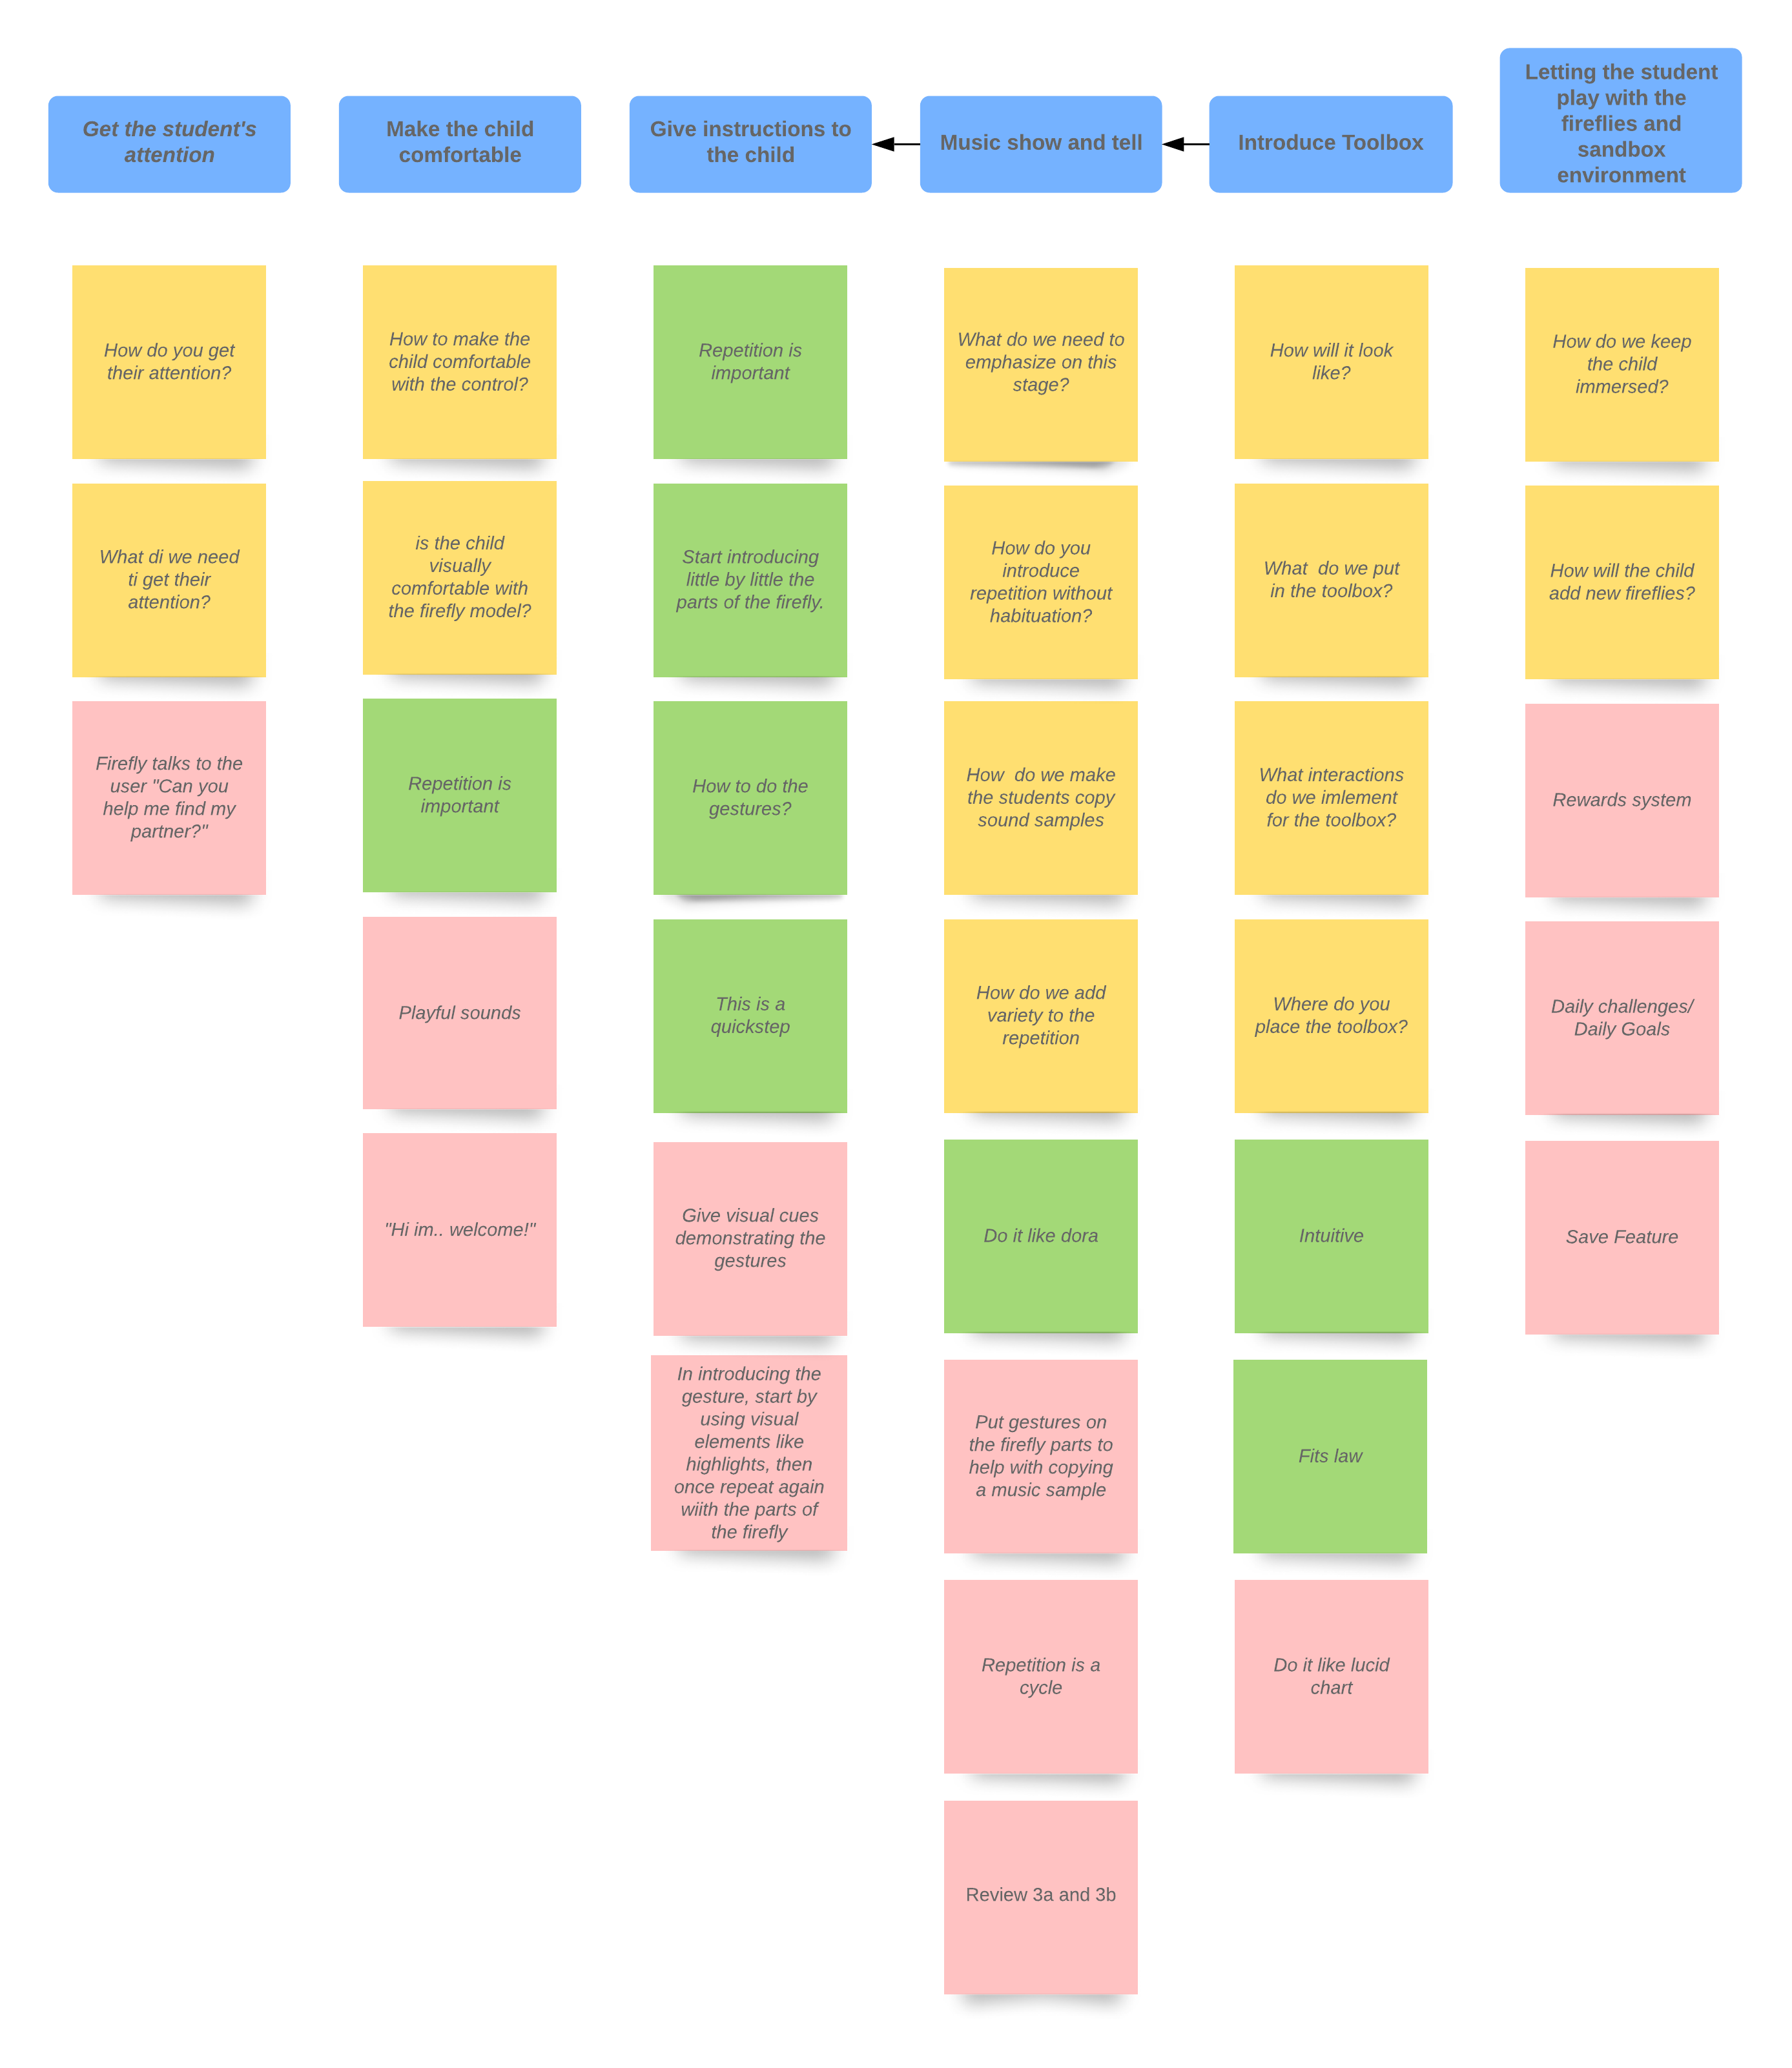
\includegraphics[width=16cm]{figures/ScenarioMaps.png}
    \label{fig:ScenarioMap}
    \caption{The digital version of the scenario map taking into account the key points from the interviews. Blue = Step, Yellow = Question, Green = Idea, Pink = Solution.}
\end{figure}

% Based on our interviews with the music teachers, we were able to hypothesize some features needed by children. These hypotheses were then clarified with them and verified. After these, it was then translated into features for the mid-fidelity prototype as shown in Table \ref{BasicFeatureTranslations}.
% \begin{table}[]
% \label{BasicFeatureTranslations}
% \caption{Basic Feature Translations. H = Hypothesis, C = Clarification,  V =Verification, T = Translation.}
% \begin{tabular}{|p{14cm}|}
% \hline
% \begin{tabular}[c]{@{}l@{}}\textbf{H:} Children would want to edit existing fireflies and explore other options or \\ settings. \\ \textbf{C:} Asked the music teacher if the child will edit existing fireflies.\\ \textbf{V:} Verified that the child would want to have the option to edit fireflies. This \\will allow the child to explore other combinations.\\ \textbf{T:} Added feature that allowed fireflies to be edited before released.\end{tabular} \\ \hline
% \begin{tabular}[c]{@{}l@{}}\textbf{H:} The child would want to replay previous tracks.\\ \textbf{C:} Asked the teacher if the child will replay previous tracks.\\ \textbf{V:} Verified that the child will want to replay previous tracks and listen \\again to the track. This will let the child to  have a clearer understanding on \\how the configurations affected the sound produced.\\ \textbf{T:} Added a feature that allowed replaying of previous tracks.\end{tabular} \\ \hline
% \begin{tabular}[c]{@{}l@{}}\textbf{H:} The child would want to save and load workspace.\\\textbf{C:} Asked the teacher if the child would want to save the existing workspace \\or load an existing workspace.\\ \textbf{V:} Verified that the child would want to save the existing workspace to allow \\them to exit the workspace anytime or load a workspace anytime. This will \\allow the child to have the freedom of continuing whenever they want to.\\ \textbf{T:} Added feature that allowed the saving of existing workspace, and loading \\of an existing workspace. \end{tabular} \\ \hline
% \begin{tabular}[c]{@{}l@{}}\textbf{H:} The child would want to reset the workspace and delete all configurations \\of the fireflies.\\ \textbf{C:} Asked the teacher if the child would want to reset the workspace.\\ \textbf{V:} Verified that the child would want to reset the workspace and reset all the \\configurations of the fireflies. This will allow the child to quickly get rid of all \\the configurations and start from scratch.\\ \textbf{T:} Added feature that allowed resetting the workspace and delete all the \\configurations of the fireflies.\end{tabular} \\ \hline
% \end{tabular}
% \end{table}
% \section{Mid-fidelity Prototype}
% \begin{figure}[H]
%     \centering
%     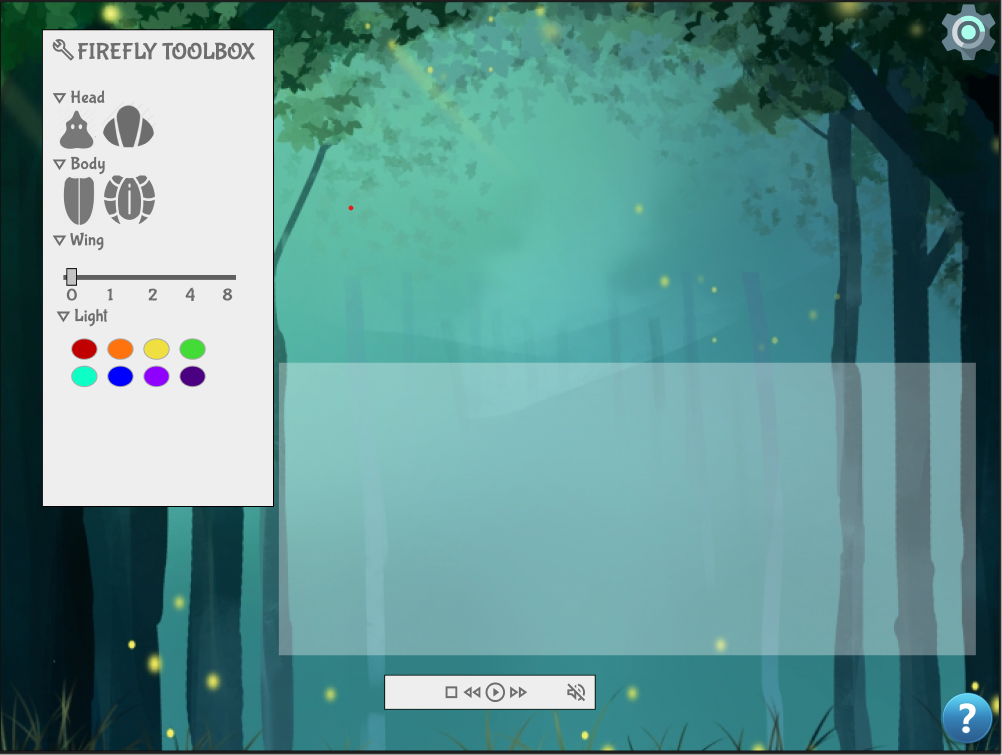
\includegraphics[width=16cm]{figures/Prototype1.png}
%     \caption{The first version of the mid-fidelity prototype built using Figma}
%     \label{fig:Prototype1}
% \end{figure}

% The mid-fidelity prototype consists of 3 spaces, namely: canvas, sandbox, and toolbox. A firefly can be built using the toolbox on the sandbox environment. The toolbox feature took inspiration from a number of applications that require drag and drop such as Lucid Chart, and Gravit. After the firefly is assembled it can be dragged on to the canvas where the firefly will roam and playback the rhythm configuration. 

% Transfer tables here in overleaf
% https://docs.google.com/document/d/1wLBHrv6spsFyLCrxCDzhwrFCYW9UCK_8IP80yTavOrM/edit
